\section{Лекція 7: Словники та кортежі}
 
 \subsection{Що таке словник?} 
\begin{frame}
% \frametitle{Логічні висновки}
Словник – невпорядкована структура даних, що дозволяє зберігати пари «ключ – значення». Їх іноді ще називають асоціативними масивами чи хеш-таблицями.

\begin{figure}
\begin{center}
 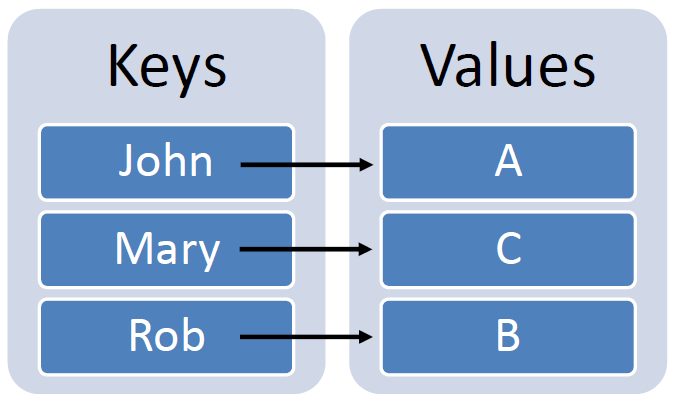
\includegraphics[width=0.4\textwidth]{pictures/dict.png}
\caption{Словник}
\label{dict} 
\end{center}
\end{figure}

\end{frame}

\begin{frame}
% \frametitle{Логічні висновки}

\begin{itemize}
  \item 
  Приклад словника d:

 d = \{ключ\_1: значення\_1,
 
  ключ\_2: значення\_2, ... 

ключ\_N: значення\_N\}
\item Доступ до значення словника: d[ключ].

\item
Створювати словники можна за допомогою конструкції:

d = dict(ключ\_1 = значення\_1, ...

 ключ\_N = значення\_N)
 
 \item Визначення пустого словника d = \{\} або d = dict()
\end{itemize}

\end{frame}

\begin{frame}
% \frametitle{Логічні висновки}
Ключом в словнику можуть бути тільки дані незмінного типу. Значеннями можуть бути дані будь-якого типу.

\begin{itemize}
  \item Для визначення числа елементів в словнику використовується функція \texttt{len}.
  
  \item Для видалення ключа \texttt{key} та його значення із словника \texttt{d} використовується команда \texttt{del d[key]}.
  \item Для перевірки, що ключ \texttt{key} присутній в словнику \texttt{d}, використовується команда \texttt{key in d}.
  \item Для перевірки, що ключ \texttt{key} відсутній в словнику \texttt{d}, використовується команда \texttt{key not in d}.
\end{itemize}
\end{frame}

\subsection{Методи словника d} 
\begin{frame}
    \begin{itemize}
        \item<1-> \texttt{d = dict.fromkeys(lst[, val])} - створює словник d, ключами якого є елементи списку lst, необов'язковий аргумент val - значення за замовчуванням;
        \item<2-> \texttt{d.clear()} - очищує словник d;
        \item<3-> \texttt{d.copy()} - створює копію словника d (інший варіант створення копії словника - функція \texttt{dict(d)} );
        \item<4-> \texttt{d.get(key)} - отримати значення по ключу key зі словника d (на відміну від \texttt{d[key]}, при звертанні до неіснуючого ключа повертає \texttt{None} або другий параметр методу \texttt{get});
    \end{itemize}
\end{frame}

\begin{frame}
    \begin{itemize}
        \item<1-> \texttt{d.setdefaults(key[, val])} - якщо ключ key є в словнику d, то повертає значення за цим ключом, інакше повертає None (або необов'язковий параметр val) та додає до словника значення None (або необов'язковий параметр val) за ключом key;
        \item<2-> \texttt{d.pop(key[, val])} - видаляє значення за ключем key зі словника d та повертає це значення, для неіснуючого ключа key повертає помилку або необов'язковий параметр val;
        \item<3-> \texttt{d.popitem()} - видаляє та повертає значення за випадковим ключем зі словника d;
    \end{itemize}
\end{frame}

\begin{frame}
    \begin{itemize}
        \item<1-> \texttt{d.keys()} - повертає список ключів словника d;
        \item<1-> \texttt{d.values()} - повертає список значень словника d;
        \item<1-> \texttt{d.items()} - повертає список кортежів із ключів та значень словника d;
        \item<2-> \texttt{d.update(d1)} - оновлює словник d значеннями зі словника d1;
        \item<3-> \texttt{d = \{**d1, **d2\}} - поєднання словників d1 та d2 у словник d.
    \end{itemize}
\end{frame}


 \subsection{Що таке кортеж?} 
\begin{frame}
% \frametitle{Логічні висновки}
Кортеж (turple) – впорядкована, але незмінна колекція довільних даних.

\begin{figure}
\begin{center}
 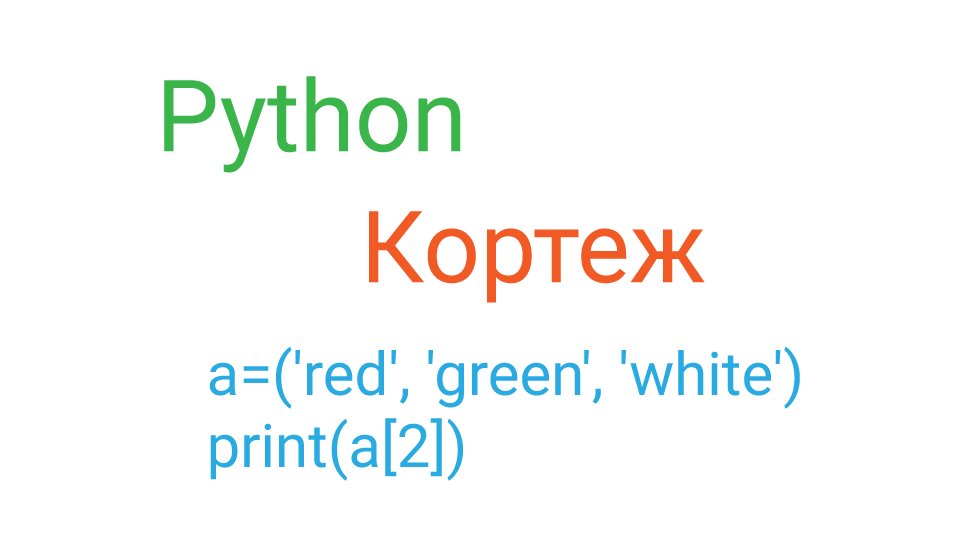
\includegraphics[width=0.4\textwidth]{pictures/turple.png}
\caption{Кортеж}
\label{turple} 
\end{center}
\end{figure}

\end{frame}

\begin{frame}
% \frametitle{Логічні висновки}
Для створення кортежу треба вказувати кому, дужки не є обов'язковими. Варіанти створення кортежу:

\begin{itemize}
  \item a = (1, 2, 3)
  \item a = 1, 2, 3
  \item a = (1,)
  \item a = 1,
\end{itemize}

Розпакування кортежу в змінні:

x, y = (1, 2)
\end{frame}

 \subsection{Функції для роботи з кортежами} 
\begin{frame}
% \frametitle{Логічні висновки}
\begin{itemize}
  \item \texttt{len(t)} - знаходження довжини  кортежу \texttt{t};
  \item \texttt{t[i]} - звертання до \texttt{i}-го елементу  кортежу \texttt{t};
  \item \texttt{t[:i:j]} - зрізи працюють так само як і для списків, лише операція \texttt{t[:]} не створює копію, а посилається на той самий кортеж \texttt{t};
  \item в кортежах не можна змінювати дані \texttt{t[i] = j} - помилка;
  \item кортежі можна використовувати як ключі словників;
\end{itemize}

\end{frame}

\begin{frame}
% \frametitle{Логічні висновки}
\begin{itemize}
  \item \texttt{t = ()} або \texttt{t = turple()} - створення пустого кортежу;
  \item \texttt{t + (1,)} - додавання елементу до кортежу;
  \item \texttt{(1,)*n} - дублювання елементів кортежу \texttt{n} разів;
  \item \texttt{turple(it)} - створює кортеж із елементів будь-якого ітерованого об'єкту \texttt{it};
  \item \texttt{val in t} - перевіряє чи ходить елемент \texttt{val} в кортеж \texttt{t}.
\end{itemize}

\end{frame}

\subsection{Методи кортежу t} 
\begin{frame}
    \begin{itemize}
        \item<1-> \texttt{t.count(val)} - повертає число знайдених елементів із значенням \texttt{val};
        \item<2-> \texttt{t.index(val, start, stop)} - повертає індекс першого знайденого елементу із значенням \texttt{val}, \texttt{start} та \texttt{stop} індекси початку та кінця пошуку (необов'язкові параметри).
    \end{itemize}
\end{frame}

 \subsection{Що таке множина?} 
\begin{frame}
% \frametitle{Логічні висновки}
Множина (set) – невпорядкована колекція унікальних елементів.

\begin{figure}
\begin{center}
 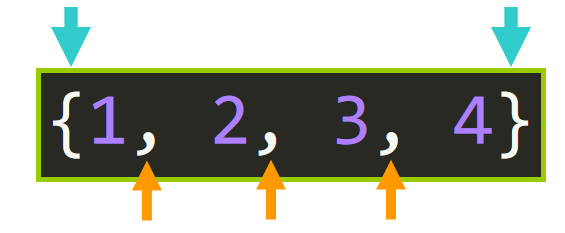
\includegraphics[width=0.4\textwidth]{pictures/set.png}
\caption{Множина}
\label{set} 
\end{center}
\end{figure}

\end{frame}

\begin{frame}
% \frametitle{Логічні висновки}
\begin{itemize}
  \item \texttt{a = \{1, 2, 3, "hello"\}} - множина;
  \item елементи множини - незмінні типи даних (числа, булеві значення, рядки, кортежі);
  \item не можуть бути елементами множин - списки, словники, інші множини;
  \item \texttt{s = set()} - пуста множина;
  \item \texttt{s = set(it)} - створює множину із унікальних елементів ітерованого об'єкту \texttt{it};
  \item звернутися до елементу множини за індексом неможливо;
  \item множина - ітерований об'єкт.
\end{itemize}

\end{frame}

 \subsection{Функції для роботи з множиною} 
\begin{frame}
% \frametitle{Логічні висновки}
\begin{itemize}
  \item \texttt{len(s)} - повертає кількіть елементів у множині \texttt{s};
  \item \texttt{val in s} - перевірка чи присутній елемент \texttt{val} у множині \texttt{s};
  \item \texttt{s.add(val)} - додає елемент \texttt{val} у множину \texttt{s};
  \item \texttt{s.update(it)} - додає елементи ітерованого об'єкту \texttt{it} у множину \texttt{s};
\end{itemize}
\end{frame}

\begin{frame}
% \frametitle{Логічні висновки}
\begin{itemize}

  \item \texttt{s.discard(val)} - видаляє елемент \texttt{val} із множини \texttt{s} (якщо елемент \texttt{val} відсутній у множині \texttt{s} - нічого не повертає);
  \item \texttt{s.remove(val)} - видаляє елемент \texttt{val} із множини \texttt{s} (якщо елемент \texttt{val} відсутній у множині \texttt{s} - повертає помилку);
  \item \texttt{s.pop()} - повертає та видаляє довільний елемент із множини \texttt{s} ;
  \item \texttt{s.clear()} - видаляє всі елементи із множини \texttt{s}.
\end{itemize}

\end{frame}

 \subsection{Операції над множинами} 
\begin{frame}
% \frametitle{Логічні висновки}
\begin{itemize}
  \item \texttt{s1 \& s2} (або \texttt{s1.intersection(s2)}) - повертає множину, що є перетином множин \texttt{s1} та \texttt{s2};
  \item \texttt{s1 = s1 \& s2} (або \texttt{s1 \&= s2} або \texttt{s1.intersection\_update(s2)}) - записує до множини \texttt{s1} множину, що є перетином множин \texttt{s1} та \texttt{s2};
  \end{itemize}
 \begin{figure}
\begin{center}
 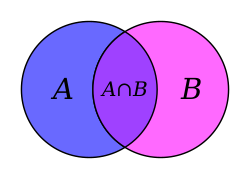
\includegraphics[width=0.25\textwidth]{pictures/intersection.png}
\caption{Перетин множин}
\label{intersection} 
\end{center}
\end{figure} 
  
\end{frame}

\begin{frame}
% \frametitle{Логічні висновки}
\begin{itemize}
    \item \texttt{s1 | s2} (або \texttt{s1.union(s2)}) - повертає множину, що є об'єднанням множин \texttt{s1} та \texttt{s2};
  \item \texttt{s1 = s1 | s2} (або \texttt{s1 |= s2} ) - записує до множини \texttt{s1} множину, що є об'єднанням множин \texttt{s1} та \texttt{s2};
\end{itemize}
 \begin{figure}
\begin{center}
 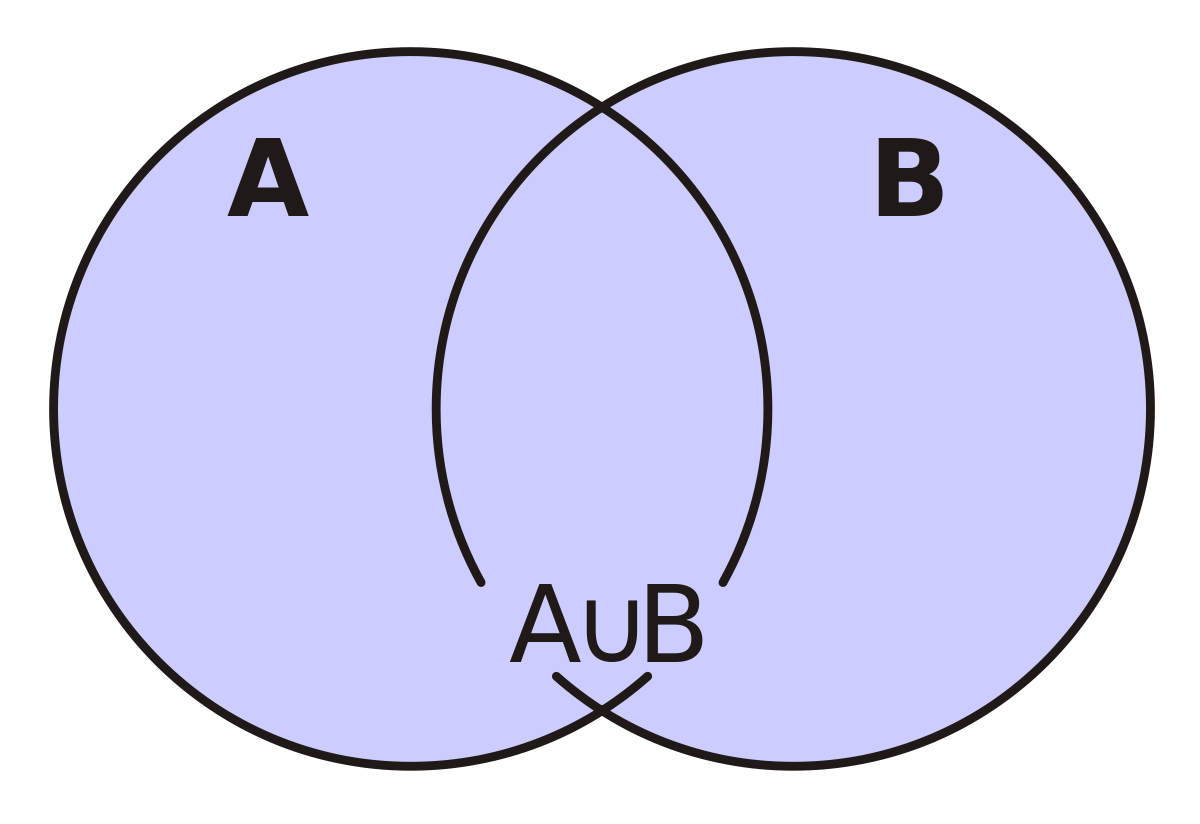
\includegraphics[width=0.25\textwidth]{pictures/union.png}
\caption{Об'єднання множин}
\label{union} 
\end{center}
\end{figure} 
\end{frame}

\begin{frame}
% \frametitle{Логічні висновки}
\begin{itemize}
    \item \texttt{s1 - s2} - повертає множину, що є різницею множин \texttt{s1} та \texttt{s2};
  \item \texttt{s1 -= s2} - записує до множини \texttt{s1} множину, що є різницею множин \texttt{s1} та \texttt{s2};
\end{itemize}
 \begin{figure}
\begin{center}
 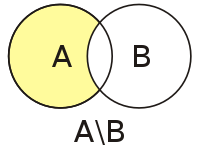
\includegraphics[width=0.25\textwidth]{pictures/subtract.png}
\caption{Різниця множин}
\label{subtract} 
\end{center}
\end{figure} 
\end{frame}

\begin{frame}
% \frametitle{Логічні висновки}
\begin{itemize}
    \item \texttt{s1 $\hat{}$ s2} - повертає множину, що є симетричною різницею множин \texttt{s1} та \texttt{s2};
%   \item \texttt{s1 -= s2} - записує до множини \texttt{s1} множину, що є різницею множин \texttt{s1} та \texttt{s2};
\end{itemize}
 \begin{figure}
\begin{center}
 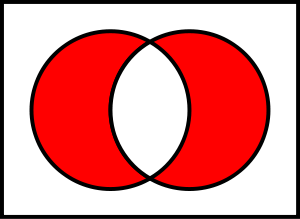
\includegraphics[width=0.25\textwidth]{pictures/xor.png}
\caption{Симетрична різниця множин}
\label{xor} 
\end{center}
\end{figure} 
\end{frame}

\begin{frame}
\frametitle{Порівняння множин}
Множини є рівними, якщо їх довжина та значення елементів співпадають. Множина \texttt{s1} входе в множину \texttt{s2}, якщо всі елементи множини \texttt{s1} містяться в більшій множині \texttt{s2}.
\begin{itemize}
    \item \texttt{s1 == s2} (\texttt{s1 != s2}) - перевірка на рівність (нерівність) множин;
    \item \texttt{s1 < s2} - перевірка, що множина \texttt{s1}  входе у множину \texttt{s2};
    \item \texttt{s1 <= s2} - перевірка, що множина \texttt{s1}  входе у множину \texttt{s2}, або вони є рівними.
\end{itemize}
\end{frame}
